\chapter{Introduction}
\begin{quote}
“Let each man exercise the art he knows” 
\end{quote}


\begin{figure}[htbp]
\begin{center}
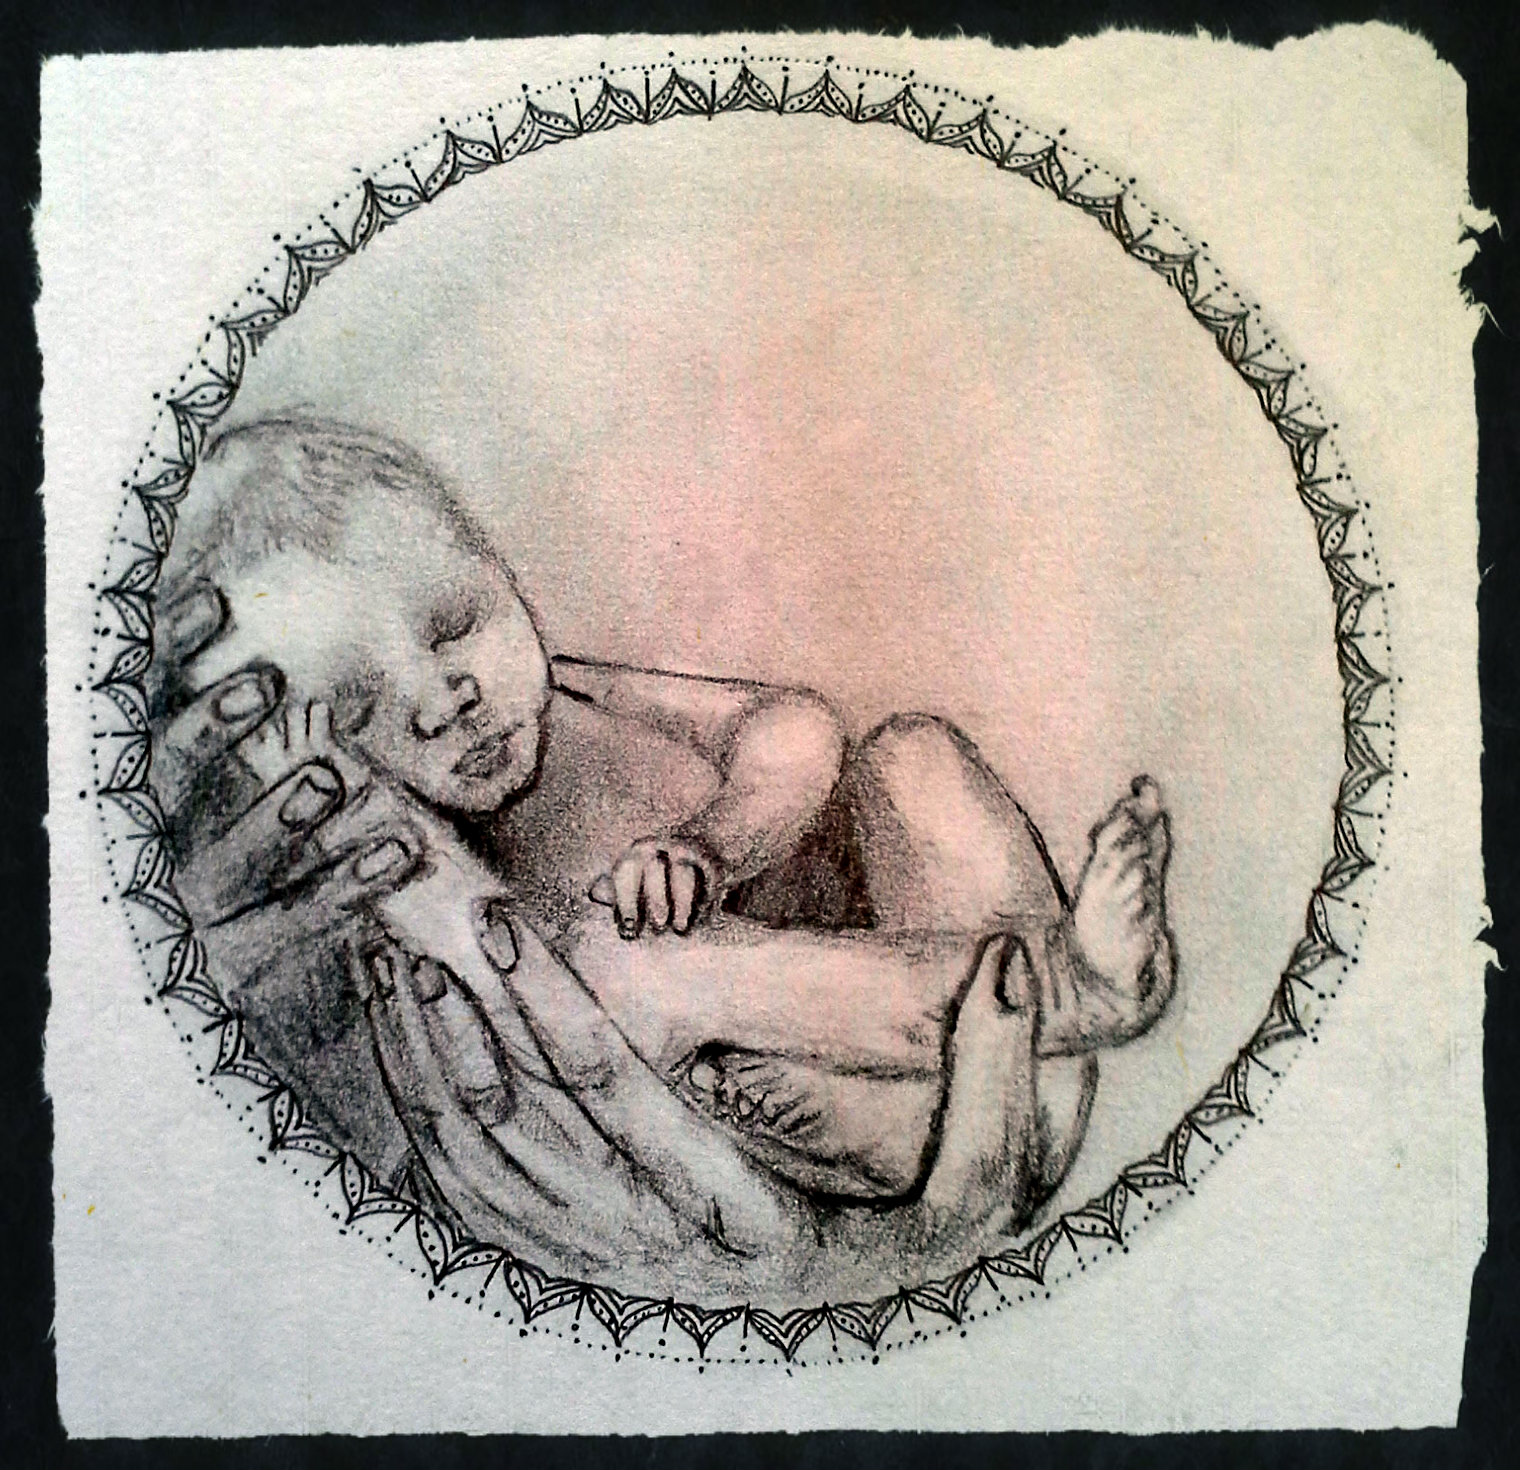
\includegraphics[scale=.25]{../eps/babymandala_1.eps} 
\caption{The birth of creating}
\label{label}
\end{center}
\end{figure}

%\begin{quote}
%"Let each man exercise the art he knows"
%\end{quote}

\newpage 


For many years mandalas have been a huge part of my life. I have been creating mandalas since 2003, when I was first introduced to the Jungian perspective on mandalas and the transpersonal approach. I have used mandalas in my private practice, provided workshops in Cambodia and have and will continue to use mandalas as a reflective tool. Consequently, all my experiences have led to my inquiry into conversations within mandalas.

I studied Fine Arts at the University of Maryland in the United States of America between 1998-2001 on a hockey scholarship and was highly influenced by abstract expressionism. As a result, I painted mainly expressionistic oil portraits and abstract paintings.


\begin{figure}[htbp]
\begin{center}
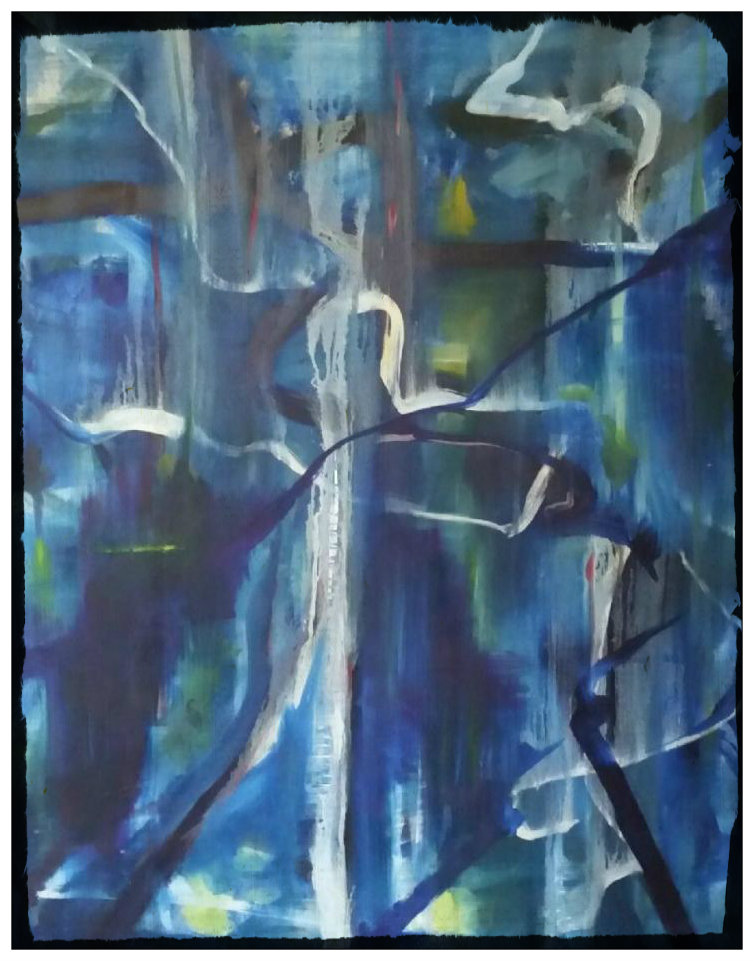
\includegraphics[scale=.25]{../eps/FIRST_ABSTRACT_PAINTING.eps}
\caption{FIRST ABSTRACT PAINTING, UNTITELED}
\label{label}
\end{center}
\end{figure}
\newpage 

\begin{figure}[htbp]
\begin{center}
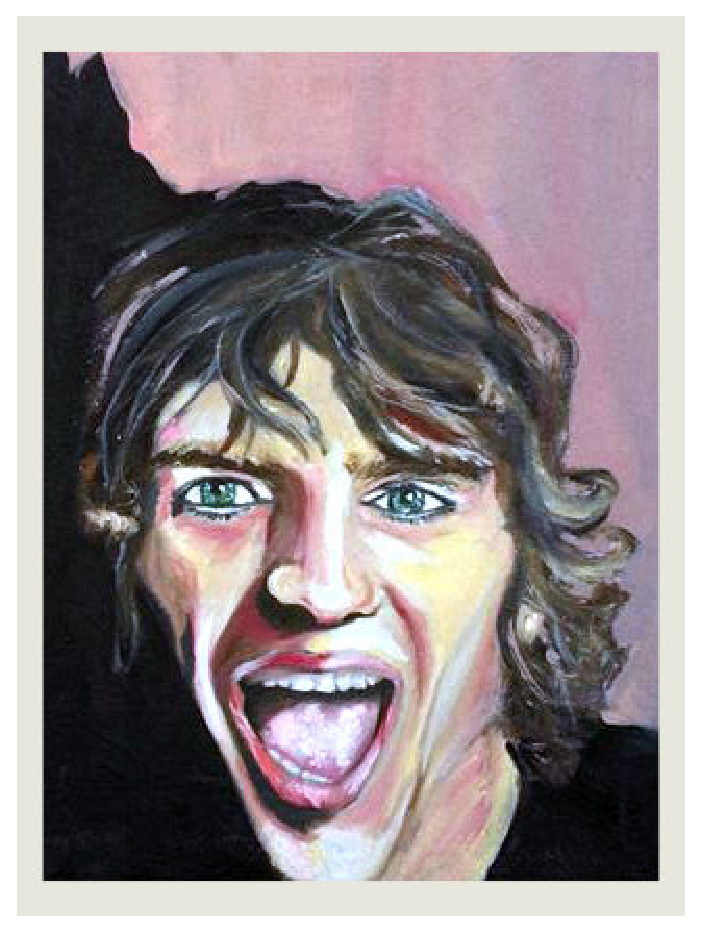
\includegraphics[scale=.50]{../eps/face.eps} 
\caption{ABSTRACT PORTITURE- UNTITELED}
\label{label}
\end{center}
\end{figure}

Abstract expressionism taught me to let go of the end result and focus on the movement of the paint and the way I felt. Hence this allowed me to be flexible in the way I created mandalas, as I let the materials dictate what was being created and I was not fixed on the end result. In this process I was able to focus on the detail whilst being playful and I felt free to make mistakes. Mandalas have always made sense to me, as they give me a sense of relief from my emotional content that builds within me and feels difficult to hold.

My former partner and I lived and worked in Australia for 9 years before moving to Cambodia for 3 years. I was working as an Arts Therapist and Counsellor, both in voluntary and paid positions, amongst other jobs to pay the bills in Cambodia. For two and a half years I worked with the Ragamuffin Project in Cambodia where we supported children and young people with multi complex traumas. I also worked with Indigo Psychological Services, where we worked with western clients; both were amazingly powerful and depressing. 

My work supervisor Carrie Herbert, encouraged me to look after myself by using experiential art mediums and keeping case notes brief and succinct. Having permission to create and attend to my self-care through using a medium that made complete sense emotionally, physically and psychologically was liberating, and intensified my passion for mandalas. I then started to use mandalas as a self-reflective and debriefing tool, along with supervision and writing case notes. I mostly kept a small sketch book of mandalas, as I regularly travelled a lot. Every second weekend I would catch a six-hour bus ride to the Province so I needed to pack light, as it was only for two nights. I also felt that minimising the actual size of the mandalas was important due to time factors that also helped to get to the essence of my experience for that session or day.
I yearned for further professional development and wanted to advance my qualifications whilst living in Cambodia. After returning to Australia with the mission of undertaking my masters. I noticed mandalas were always at the forefront of my awareness and I was conscious that there was something really important to explore and inquire into but I did not know why.

\section{Beginning my inquiry}

When I began my exploration, I was interested in the two following topics:
\begin{itemize}
\item mandalas, because I feel connected to the process. 
\end{itemize}

\begin{itemize}
\item emotions, mainly because I feel we are so out of touch most of the time. 
\end{itemize}

However, I quickly realized that emotions naturally are a part of the process of inquiring into creating a mandala. So essentially, I was inquiry into the two things that I held important to explore through my Masters process.  
My supervisor Dr Jan Allen suggested that I take a few different angles as I inquired into the process of creating mandalas.

\newpage

\begin{enumerate}
\item Drawing a mandala whilst tracking and writing all my thoughts, sensations, emotions and memories down 
\item Drawing a mandala and then dialoguing with it 
\item Drawing a mandala and then using MIECAT methods of inquiry to explore my understanding 
Initially, I mainly drew mandalas which tracked my emotions, thoughts, sensations and memories. I enjoyed slowing down all my thoughts and feelings, I became lost in the stillness at times and then took a breath back into the present feeling, memory and emotions. 
\end{enumerate}














